\section{茶和咖啡的碰撞}
茶和咖啡都是现代生活中最常见,最普通的饮品。中德工程师学院也常常举办咖啡吧活动,邀请德国留学生参与游戏,让大家在香醇的咖啡中,了解德国文化。 

谈到喝,那就要说一下,我们什么时候喝茶和咖啡,在哪喝茶和咖啡。简而言之就是各自的饮用场合。作为世界茶叶的发源地之一,中国人从古自今就十分喜欢喝茶。如在家难得清闲时,会泡上一壶清茶独自享受一下生活;同样以茶待客是中国人的一种习惯,客人进门,主人立即送上一杯香气扑鼻的茶水,边喝茶边谈话,气氛轻松愉快;在茶楼中喝茶现在也是比较常见的,双方有什么事情或者生意也会在茶楼里边喝茶边谈。
位于大洋彼岸的德国人其实也是很爱喝茶的。但是相较于中国,德国没有专门卖茶水的茶楼。德国人喜欢在阳光明媚的午后,在自家的庭院中,沏一杯茶饮用。其实茶和咖啡对于德国人只是一种个人喜好的选择,无论是茶还是咖啡,配上一些糕点,就是一份精致的下午茶。咖啡在中国虽然像茶一样常见,但是饮用场合还是有一些区别的。中国人一般是在上班工作的时候或者一些快捷的咖啡馆里喝一杯咖啡,振奋一下自己,提高自己的工作效率。咖啡在中国更像是一种快餐式消费。
\begin{figure}
    \centering
    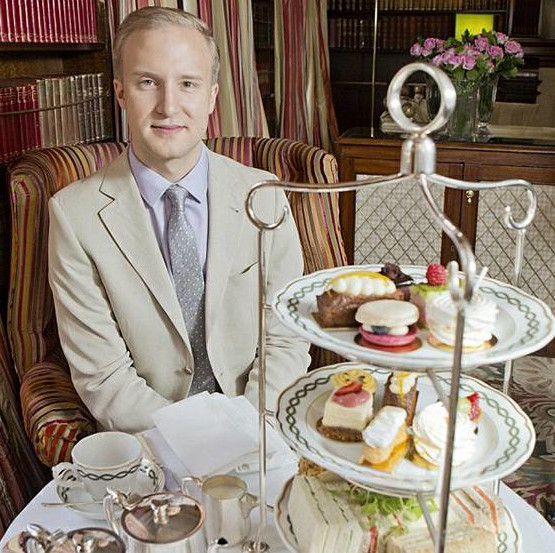
\includegraphics[width=0.4\linewidth]{Tee}
    \caption{日常下午茶}
\end{figure}
饮茶的风气在中国盛行,且历史悠久,距今已有4千多年的历史,在唐-陆羽《茶经》记载:“茶之为饮,发乎神农氏”。中国也是最懂得饮茶真趣,以茶待客、以茶会友、以茶联谊等历来是我国各民族的饮茶之道。这里还有一个小故事,据说在公元280年之前,中国南方有一个小国叫吴国,国王在宴请大臣时,喜爱用酒把大臣们灌醉。其中有一个叫韦昭的大臣酒量很小,国王就让他以茶代酒,从这以后,文人便开始以茶接待宾客。上文也已经提到,中国人喝咖啡除了常见的为了提高自己的工作效率,也会有如茶一样的目的,以咖啡会友等。
在德国,喝茶喝咖啡都一样,都是一种享受生活的方式,同样也会有会友的作用,唯有双方关系不错,才会邀请对方来家中一起喝下午茶。

中国人在日常生活中不可缺少的饮料之一就是茶,俗话说“柴、米、油 、盐、酱、醋、茶”,茶被列入开门七件事之一,可以看出喝茶的重要。茶之于中国人有极多的文化含义,如包含有儒家之礼,佛家之养,道家之闲。最具代表性的即是茶道,他体现了中国人喝茶的仪式感,追求的是一种君子之德。茶道,就是品赏茶的美感之道。亦被视为一种烹茶饮茶的生活艺术,一种以茶为媒的生活礼仪,一种以茶修身的生活方式。它通过沏茶、赏茶、闻茶、饮茶、增进友谊,美心修德,学习礼法,领略传统美德,是很有益的一种和美仪式。喝茶能静心、静神,有助于陶冶情操、去除杂念。
几百年来,咖啡这种醇香的苦涩吸引着各色各样的人们,并因此渗透于西方近代社会的各个领域,似血液一般流淌在欧洲大地,流淌过了几个世纪。如今,它已经成为西方文化的典型代表。咖啡对于西方人来说更多是享受环境和情调,代表着一种浪费惬意的文化追求。它是众多西方作家的良友,巴尔扎克在写下《人间喜剧》的同时,一生豪饮咖啡5万杯;荷兰后印象派画家凡•高痴迷于咖啡馆中上演的世间百态,一次次推开阿尔加萨咖啡馆夜间仍旧开着的门,用画笔记录下咖啡馆内的情景;德国音乐家巴赫以咖啡为题材的作品《第211号康塔塔》,也被称作《咖啡康塔塔》(康塔塔:大型声乐套曲体裁的一种),达到了咖啡与音乐的完美结合;著名哲学家萨特即使在二战期间空袭警报长鸣、全城一片混乱的时候,仍旧每天在巴黎双偶咖啡馆坚持写作。这样的例子还有很多。这群人有着对真理的虔诚,有着对艺术的向往,有着对美的追求,咖啡并非其作品问世的原因,但是对他们来说却是何等的重要!
